\documentclass{llncs}
\RequirePackage[english]{babel} % Se fizerem o texto em ingles
\usepackage[english]{babel}   
%\usepackage[latin1]{inputenc}
\usepackage[utf8x]{inputenc}
\usepackage[T1]{fontenc}

\usepackage[fleqn]{amsmath}
\usepackage{amssymb}
\usepackage{makeidx}  % allows for indexgeneration
\usepackage{subfig}  % allows for indexgeneration
\usepackage{color}  % allows for indexgeneration
\usepackage{url}
\usepackage{hyperref}
\usepackage{float}
\usepackage{mathtools}
\usepackage{acronym}
\usepackage{pgfgantt}
\usepackage{adjustbox}
\usepackage{rotating}
\usepackage{dirtytalk}
\usepackage[graphicx]{realboxes}
\definecolor{fade}{rgb}{0.8,0.8,0.8}


\newacro{AES}{Advanced Encryption Standard}
\newacro{API}{Application Programming Interface}
\newacro{BOSH}{Bidirectional-streams Over Synchronous HTTP}
\newacro{CBC}{Cipher Block Chaining}
\newacro{CPU}{Central Processing Unit}
\newacro{CRUD}{Create, Read, Update and Delete}
\newacro{CSS}{Cascading Style Sheets}
\newacro{DOM}{Document Object Model}
\newacro{DTLS}{Datagram Transport Layer Security}
\newacro{DVD}{Digital Versatile Discs}
\newacro{FMS}{Flash Media Server}
\newacro{HTML}{HyperText Markup Language}
\newacro{HTTP}{Hypertext Transfer Protocol}
\newacro{ICE}{Interactive Connectivity Establishment}
\newacro{IPv4}{Internet Protocol Version 4}
\newacro{IPv6}{Internet Protocol Version 6}
\newacro{IP}{Internet Protocol}
\newacro{JSON}{JavaScript Object Notation}
\newacro{MPEG}{Moving Picture Experts Group}
\newacro{MVC}{Model-View-Controller}
\newacro{NAT}{Network Address Translation}
\newacro{OT}{Operational transformation}
\newacro{P2P}{Peer-to-peer}
\newacro{PSTN}{Public Switched Telephone Network}
\newacro{RFC}{Request For Comments}
\newacro{RTCP}{Real Time Control Protocol}
\newacro{RTSP}{Real Time Streaming Protocol}
\newacro{RTMFP}{Real-Time Media Flow Protocol}
\newacro{RTMP}{Real Time Messaging Protocol}
\newacro{RTP}{Real-time Transport Protocol}
\newacro{SAMI}{Synchronized Accessible Media Interchange}
\newacro{SCTP}{Stream Control Transmission Protocol}
\newacro{SDP}{Session Description Protocol}
\newacro{SigOfly}{Signaling-On-the-fly}
\newacro{SIMPLE}{SIP for Instant Messaging and Presence Leveraging Extensions}
\newacro{SIP}{Session Initiation Protocol}
\newacro{SMIL}{Synchronized Multimedia Integration Language}
\newacro{SMS}{Short Message Service}
\newacro{SRTCP}{Secure RTCP}
\newacro{SRTP}{Secure Real-time Transport Protocol}
\newacro{SRT}{SubRip Text}
\newacro{SSL}{Secure Sockets Layer}
\newacro{STUN}{Session Traversal Utilities for NAT}
\newacro{SVG}{Scalable Vector Graphics}
\newacro{TCP}{Transmission Control Protocol}
\newacro{TLS}{Transport Layer Security}
\newacro{TMN}{This Means Nothing}
\newacro{TURN}{Traversal Using Relays around NAT}
\newacro{UDP}{User Datagram Protocol}
\newacro{VoIP}{Voice Over IP}
\newacro{WebRTC}{Web Real-Time Communication}
\newacro{WebVTT}{Web Video Text Tracks}
\newacro{XAML}{eXtensible Application Markup Language}
\newacro{XEP}{XMPP Extensions}
\newacro{XHTML}{eXtensible Hypertext Markup Language}
\newacro{XML}{eXtensible Markup Language}
\newacro{XMPP}{Extensible Messaging and Presence Protocol}

%\overfullrule=2cm



\newganttchartelement*{mymilestone}{
mymilestone/.style={
shape=isosceles triangle,
inner sep=0pt,
draw=cyan,
top color=white,
bottom color=cyan!50
},
mymilestone incomplete/.style={
/pgfgantt/mymilestone,
draw=yellow,
bottom color=yellow!50
},
mymilestone label font=\slshape,
mymilestone left shift=0pt,
mymilestone right shift=0pt
}

\newgantttimeslotformat{stardate}{%
\def\decomposestardate##1.##2\relax{%
\def\stardateyear{##1}\def\stardateday{##2}%
}%
\decomposestardate#1\relax%
\pgfcalendardatetojulian{\stardateyear-01-01}{#2}%
\advance#2 by-1\relax%
\advance#2 by\stardateday\relax%
}



\begin{document}
\pagestyle{plain}
\mainmatter              % start of the contributions

\title{Hyper-linked Communications: WebRTC enabled asynchronous collaboration}
\author{%
	Henrique Duarte Lopes Rocha \\
	email1: henrique.rocha@tecnico.ulisboa.pt \\
  email2: hdlopesrocha91@gmail.com \\
  student number: 68621
}
\institute{Master Degree in Telecommunications and Informatics Engineering \\ Instituto Superior Técnico \\ Universidade de Lisboa}
%RP acrescenta número de aluno, nome do mestrado e ``cadeira de projecto''
\maketitle              % typeset the title of the contribution

\begin{abstract}
Hyper-linked communications concept applies much of the hypermedia concepts, widely used on Web content, for communication and collaboration services. This paradigm allows to synchronize and structure the communications content, providing a way to integrate social media content and collaborative tools into voice and video calls.

Voice and image together can express emotions and expose creativity like no other medium can. With hypermedia concepts we can add more value to voice and video communications.

WebRTC technology, allows real-time communications between web browsers without being forced to install and use additional applications or plug-ins. The nature of web browser applications already follow the hypermedia concept, which makes WebRTC the ideal technology to apply the hyper-linked communications concepts.

The native support of WebRTC in operating systems extends its usage to outside the web browser, allowing to explore functionalities that browsers are poor to support such as video recording and massive information storage.

Our goal in this project is to develop an application that applies Hyper-linked communications concept using WebRTC.

\keywords{WebRTC, asynchronous, communications, collaboration}
\end{abstract}

\section{Introduction}
  \subsection{Context}   % English
Since the early days of Human History, we tried to communicate over far locations, from smoke signals to letters delivered by messengers. Real-time communications were limited or even nonexistent. Despite all the efforts made to improve communications, written communication could never replace face to face communication.
With the advent of the telephone network, communications have taken a very important step for us to feel more connected with whom we communicate. Still, only the human voice was not enough, and the invention of cameras and consequent video digitization were a huge step for real-time communications.

	In the past, handwritten documents were limited to a writer per page at a time. Writing a book collaboratively was a difficult task due to synchronism between writers.
	Today, we can achieve more, it is possible to write a document collaboratively, correct spelling mistakes without wasting paper, restructure text at any moment, add a video to a newspaper article and more. Although much of what was said seems banal nowadays, none of this was possible before the computer's invention. 

	As Martin Geddes states\cite{geddes}, \say{No computer in our lifetimes will ever rival a human voice’s capacity to conveying rich and complex social and emotional meaning} , although nothing replace the physical contact with a person while we communicate, we are at a time when we can do more than just a visual and verbal communication, hypermedia can be added to video and voice in order to extend its value. The concept of structured voice and video synchronized with hypermedia is called hypervoice.
        %RP a citação do geddes faz sentido? Parece estar a falar de voz gerada por computador e não de video conferencia onde o que ouvimos são outras pessoas!
        
\subsection{Problem Statement} % English

	As communications technologies appeared, we adapted the way we communicate. This project don't aims to replace the current video and audio communications, but to enrich them with hyper-media content and make them a more natural and easy to learn process. 

	For multiple reasons, we often need to repeat or postpone some of our tasks, some people tend to forget what they ear or see.
               %RP acho que toda a gente se esquece eventualmente. Pode não lhe parecer importante na altura. Não é preciso estar doente!
        A real-time system is an huge source of information that requires much attention from its users, an application that provides a way to remember our past communications would be a strong tool for not only to catch what we lost but also to enhance our knowledge.
%RP estes dois ultimos pontos são melhores. Não fales em pessoas com problemas de memoria mas em termos de lidar com grandes quantidades de informação, realizarmos comunicações em grupo (ainda nãofalaste diss) e nem sempre ser possível estar presente.
        Real-time communication applications can make a difference on business, education and health sectors by providing tools for teaching and learning online, teamworking and socializing.
        %RP também há outros mercados, como online learning, projectos de longa duração que vão evoluindo e onde é preciso revisitar o que aconteceu antes. Fins histórios. Necessidade de manter registos devido a requisitos legais/registar história.

	This project aims to complement current audio, text and video communications in order to create rich and collaborative interfaces with the ability to add more content on a future time (e.g. creating annotations for improving content search) in order to increase its value. Another important aspect of this project is the ability to navigate in time and space by rewind communications, fast-forward, jump to certain points and choose another path.


                %RP esta última frase está confusa.

        %Estás muito parco nos objectivos do projecto. Acho que falta dizer que é um sistema para complementar/subsitutir actuais sistemas de comunicação audio/video real-time, adicionando-lhe a capacidade de: adicionar conteúdo posteriomente (e.g. anotações) por forma a aumentar o seu valor; permitir acesso posterior (mesmo que apenas 5 minutos depois para quem chega atrasado); permitir navegar na comunicação (hypermedia, saltos, fast-forward, rewind).

\subsection{Thesis Goals} % English

A web application with an easy to learn user interface will be developed to accomplish solving our problem. Our application, unnamed yet, is targeted at web browsers that are compatible with only standard technologies like JavaScript, \ac{WebRTC}, \ac{HTML}5 and \ac{CSS}3. Any additional plug-in is avoidable, \emph{JavaScript} libraries will be preferred as they can be downloaded on the fly.  

%RP podes elaborar um pouco. Objectivos são: realizar o levantamento do estado da arte no espaço do problema para fundamentar uma solução; apresentar uma solução e desenhar uma arquitectura para dar resposta ao problema apresentado; construir protótipo funcional; desenhar e realizar uma avaliação/testes que provem a adequação e validade dos conceitos desenvolvidos (elaborar); escrever um artigo.

Although we propose an initial solution to solve our problem, we will make a continuous effort to survey the systems that solves our problem either completely or just a part of it.

We will present an architecture that can meet our goals, implement the respective prototype and test it with real users, unitary tests and benchmarks.

According to Martin Geddes, the quality of the interaction worsens as the number of users increase\cite{geddes}. In our testing phases we will quantify and qualify the impact of increasing users on the interface and performance of our prototype. 

	All the problems faced during the development and limitations will be reported on the thesis so that a future project better then ours can be easily and better developed.
        %RP esta última frase não é muito necessária

\subsection{Document Structure} % English
This document is structured as follows. Section \ref{related} presents the related work.
%	Section \ref{early} describes the problems that real-time communications face on nowadays internet, namely the \ac{IPv4} address exhaustion and the client server model constraints. 
%	Section \ref{rtc} describes the \ac{WebRTC} technology and the protocols needed to implement our project. 
%	Section \ref{signaling} addresses the signaling component of chat applications, which is not defined on \ac{WebRTC} specifications. 
%	Section \ref{hypermedia} presents the evolution of multimedia content until the hypermedia, its capabilities, synchronization mechanisms and interactivity. 
%	Section \ref{collab} explores streaming protocols for non-interactive multimedia and how to introduce the interactive component, another important aspects are the ability to control the time flux of a stream and collaborative application development.
%RP este detalhe sobre a estrutura da sec. do estado da arte vai para o início dessa secção.   
	In Section \ref{arch}, we propose an architecture for an Web Application that fulfills the goals of this thesis, including all the need infrastructure and software.
	Section \ref{meth} describes our work methodology and our plan for implementing and validating our proposed architecture.
	Section \ref{concl} presents the summary and conclusions of our work.



\section{Related Work}\label{related}
 This section is structured as follows.
 Section \ref{early} describes the problems that real-time communications face on nowadays internet, namely the \ac{IPv4} address exhaustion and the client server model constraints. 
 Section \ref{rtc} describes the \ac{WebRTC} technology and the protocols needed to implement our project. 
 Section \ref{signaling} addresses the signaling component of chat applications, which is not defined on \ac{WebRTC} specifications. 
 Section \ref{hypermedia} presents the evolution of multimedia content until the hypermedia, its capabilities, synchronization mechanisms and interactivity. 
 Section \ref{collab} explores streaming protocols for non-interactive multimedia and how to introduce the interactive component, another important aspects are the ability to control the time flux of a stream and collaborative application development.
%RP este detalhe sobre a estrutura da sec. do estado da arte vai para o início dessa secção.
        
  \subsection{Early days of the Internet and its remaining flaws}\label{early}

The need to build a global communications network in an age when almost nobody had access to that technology and the number of future users was unpredictable, lead to some protocols not being suitable for the huge growth of users that followed. \ac{IPv4} limits the number of public addresses in such a way that today they are scarce \cite{ipv4}. One way to overcome this problem was the development of a mechanism that groups multiple address into a single one, the machine that is assigned that address is then responsible for redirecting messages to members of its group using their private addresses, each connection in the private network is identified publicly by the same \ac{IP} address with a different port.
%RP o porto não identifica uma máquina (membro da rede privada) mas uma ligação.
This technique is known as \ac{NAT}.

\begin{figure}[H]
	\centering
	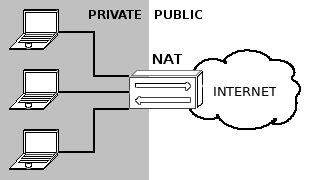
\includegraphics[width=0.6\textwidth]{figures/nat.png}
	\caption{Network Address Translation}
\end{figure}
%RP na figura devias indicar que uns tem ips publicos e outros privados. Alternativamente, colocavas metade da nat box dentro da núvem para indicar que esta pertence à Internet e os pc não. 

Initially \ac{NAT} offered an alternative to address exhaustion and a minimal sensation of security, although its current wide usage, \ac{NAT}s are exposing their weaknesses to the application layer.
%RP initially? E hoje?
There are four types of \ac{NAT} implementations\cite{rfc3489}: \emph{Full Cone NAT}, \emph{Restricted Cone NAT}, \emph{Port Restricted Cone NAT}, \emph{Symmetric NAT}.
%RP apresentas 5. falas em asymmetric. É um erro?

\emph{Full Cone} \ac{NAT} maps each public \ac{IP} address and port to a private \ac{IP} address and port.
Any external host can communicate with private hosts through their mapped public address and port. This represents the least restrictive type of \ac{NAT} and as we will later, the unique type of \ac{NAT} that enables real time communications from point to point.

\emph{Restricted Cone} \ac{NAT} requires that a private client must first send a message to an external host before it can receive messages from the same host. With this type of \ac{NAT}, the private client can be contacted from any port of the same external host.

\emph{Port Restricted Cone} \ac{NAT} works in the same way as Restricted Cone \ac{NAT}, but it only allows communications from the same external host's IP address and port, ignoring all messages from other applications within the same external host.

\emph{Symmetric} NAT maps different ports for each connection, as we will see later, this type of \ac{NAT} represents a problem on real time communications.

\emph{Full Cone}, \emph{Restricted Cone} and \emph{Port Restricted Cone} \ac{NAT}s became the common configurations on the Internet. As a direct result, problems started to appear: the amount of ports that \ac{IP} makes available is also small compared to our current needs; worse than that, \ac{NAT} also difficults end-to-end communication, forcing most applications that follow this model to be implemented ineffectively.

Applications behind a \ac{NAT} are prevented to receive incoming connections from the public network, which forces them to behave as a client of a client-server model. 

%RP explicar que o nat funciona num cenário em que a máquina atrás do nat é apenas um consumidor de informação, trabalhando em modo cliente do modelo cliente-servidor. Em P2P isto falha.

Applications based on multimedia and peer-to-peer file sharing have been one of the most strained by \ac{NAT}. Those kind of applications require real time communication in order to achieve the best performance.
%RP file sharing não precisa de real-time
\ac{STUN} and \ac{TURN} \cite{natvoip} servers are a possible solution to overcome \ac{NAT}, although, none of those can establish direct connections on multiple level \ac{NAT}s.
%HR XXX I was here
%RP explicar o que são multiple level pois não falaste disto antes? São ``nested''?

\ac{STUN} servers are quite simple. They receive requests from \ac{NAT}ed clients, with the source address of a request being the public address that \ac{NAT} mapped to the client. \ac{STUN} servers will then reply to the client, providing the mapped public address, so it knows its associated public \ac{IP} address and port. Symmetric \ac{NAT} changes \ac{IP} port for each different connection, for that reason, when the \ac{STUN} servers reply with the \ac{IP} address and port of their connection, it will be useless for clients to use in other connection connections. That is why Symmetric \ac{NAT} represents a problem for real time communications.   
%RP os problemas que relatas têm a ver com P2P ou real-time?

\ac{TURN} uses public servers to relay traffic between private endpoints.
It may use a \ac{P2P} network relay to find the best peer, but after that, the behavior is much like client-server. Direct communication is only achieved by \ac{STUN} when \ac{NAT} is a type \emph{full cone}. \ac{ICE} uses \ac{STUN} when it's possible and \ac{TURN} otherwise.
%RP ainda não explicaste o que é o ICE
%RP explicar que para usar TURN as aplicações têm de estar cientes disso.

Most of client-server applications aren't affected by \ac{NAT} when the servers are public, but they're inadequate for real time communication between two private endpoints. Clearly this type of communication requires a more expensive infrastructure and, in most cases, more network usage, leading to a worse quality of service. The requirements of real-time video communication makes this kind of model unsuitable.
%RP quando falas em infraestrutura mais dispendiosa para o video, está a falar da internet ou ainda estamos a falar de usar ICE?


When connection is established, either in a direct or indirect way (via \ac{TURN} servers), \ac{WebRTC} came to simplify how audio and video are transmitted through web browsers.

\subsection{Real time communications}\label{rtc}

\ac{WebRTC} is an open source technology that defines a collection of standard protocols and JavaScript \ac{API}s for web browser based real time communications without installing any additional application or plug-in.
%RP indicar que agora também já temos webrtc fora do browser devido ao seu sucesso e ao facto de reunir tecnologia state of the art?

\begin{figure}[H]
	\centering
	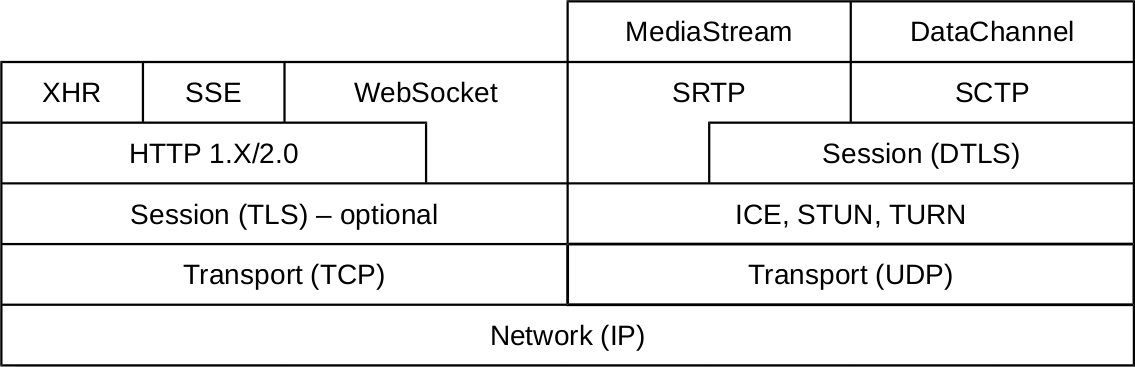
\includegraphics[width=0.9\textwidth]{figures/webrtc_stack.png}
	\caption{WebRTC protocol Stack}
\end{figure}

\ac{WebRTC} defines three main \ac{API}s: MediaStream, PeerConnection and DataChannel. 

\begin{itemize}
  \item \textbf{MediaStream} allows the browser to access the camera, microphone and the device's screen. 

  \item \textbf{PeerConnection} acquires connection data and negotiates with peers.
%RP establishes and negociates a connection with a peer for transmitting real-time video or audio?
  \item \textbf{DataChannel} provides a channel for exchanging arbitrary data with other peers.
\end{itemize}

\ac{WebRTC} uses \ac{UDP} for transporting data, which provides lower latencies than \ac{TCP}, but is not reliable and does not assure packet order and integrity. \ac{SCTP} and \ac{SRTP} are used for streaming data, providing a mechanism for congestion control and partial reliable delivery over \ac{UDP}. All transferred audio, data and video must be encrypted with \ac{DTLS} symmetric keys. \ac{DTLS} provides the same security guarantees as \ac{TLS}. 

\ac{TLS} doesn't support independent record decryption, for that it requires a reliable transport channel, typically \ac{TCP}. The decryption of a record depends on the previous record, which for unreliable transport protocols like \ac{UDP} may represent a problem, either due to packet loss or different reception order.

\ac{DTLS} is similar to \ac{TLS}, but is used on top of \ac{UDP}.
The main difference is the inclusion of a sequence number per packet that is used for packet re-ordering on reception and protects from duplicated packets. If a packet sequence number is less than the expected sequence number the packet is discarded. If a packet sequence number is greater than the expected sequence number the packet may be enqueued or discarded. By knowing the sequence of messages that are sent and received in \ac{TLS}, timers are used for packet retransmission avoiding acknowledgment messages.
%RP TLS?

\begin{figure}[H]
	\centering
	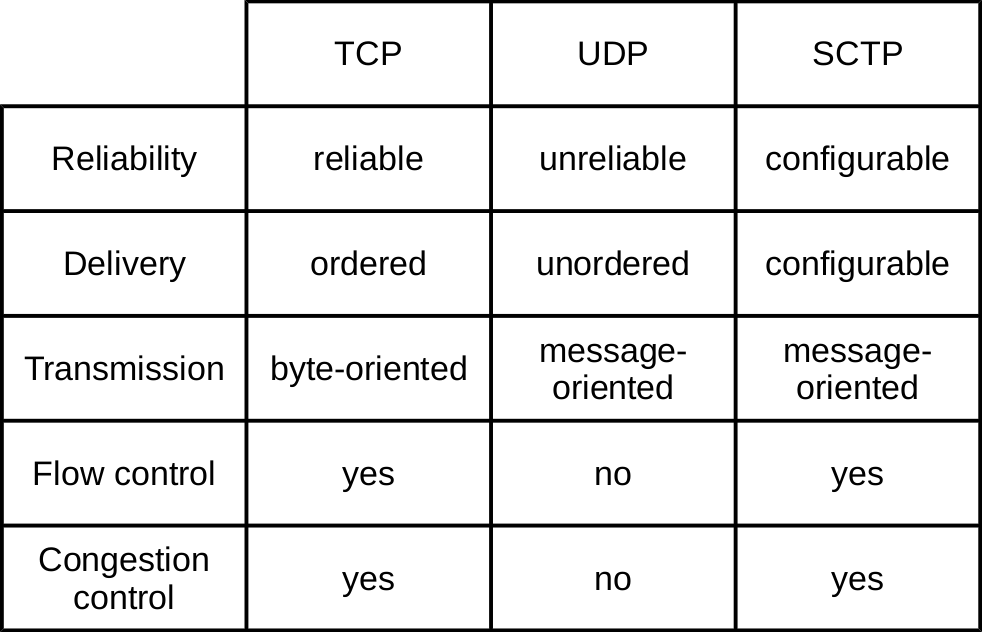
\includegraphics[width=0.6\textwidth]{figures/basic_protocols.png}
	\caption{Overview of transport protocols}
\end{figure}

\ac{WebRTC}'s \emph{DataChannel} is built on top of \ac{SCTP}, which is encapsulated by \ac{DTLS}. \ac{DTLS} encapsulation provides confidentiality, authentication and integrity to the transfered data. A \emph{Data Channel} has one incoming stream and one outgoing stream, providing bidirectional communication. Each data channel direction can be configured for reliable or unreliable transmission, the same can be done for order delivery and priority. which can also be defined for improving the quality of service of a particular stream over the others.

\ac{WebRTC}'s \emph{MediaStream} is built on top of \ac{SRTP}, which requires an external mechanism for key exchange. \ac{DTLS} keys are negotiated on handshake in order to achieve a secure connection. The new keys derived from \ac{DTLS} handshake are seized for \ac{SRTP} encryption, the remaining communications are done through \ac{UDP} without using \ac{DTLS}.
%RP quais remaining?  A última frase é confusa

\ac{WebRTC} aims to provide a standard platform for real-time audio and video on the Web. It arrives at a time when several proprietary products are well established.
\emph{Skype}\footnote{\url{http://www.skype.com/}} is an application that allows video, voice and instant messaging communication over proprietary protocols, its main strength is the amount of users that are using it nowadays. But compared to \emph{Skype}, \ac{WebRTC} applications don't need to be pre-installed.

\emph{Google Hangouts}\footnote{\url{http://plus.google.com/hangouts}} is another popular video conference web application.
In the past, in order to use \emph{hangouts} on a web browser a plug-in had to be installed, nowadays hangouts is using \ac{WebRTC}.

\emph{Jitsi Meet}\footnote{\url{http://jitsi.org/Projects/JitsiMeet}} is a \ac{WebRTC} collaborative application that uses \emph{Jitsi Videobridge} for high quality and scalable video conferences and supports shared document editing. \emph{Jitsi Videobridge} is a server that enables multi-party video calls.

%RP a descricção do skype, hangouts e jistsi cai um pouco do céu. Não há uma transição e não é feita uma análise. Apenas são indicados. Não há comparação entre eles nem com o que pode ser feito por webrtc.



  \subsection{Signaling, meet and get to know}


  Signaling is the most important process for applications to exchange connection information about peers and servers, their capabilities and meta-data.

  \ac{WebRTC} doesn't implement signaling, different applications may require different protocols, there is no single answer that fits all problems. Amongst multiple options, signaling can be done by using \ac{SIP}, \ac{XMPP}, \emph{WebSockets}, \emph{Socket.io} or by implementing a custom protocol.

  \ac{WebRTC} uses \ac{SDP} \cite{rfc4566} to define peer connection properties such as types of supported media, codecs, protocols used and network information. An \ac{SDP} offer describes to other peers the expected type of communication and its details, such as used transport protocols, codecs, security and other.

  One of signaling requisites is bi-directional communication over \ac{HTTP}. \ac{HTTP} works on a request followed by a server response, by other words, follows a unidirectional communication. Sometimes it's required that some informations are obtained in real time, as we saw, some \ac{NAT}'s don't support callbacks from servers, one technique to overcome this problem is polling.

  Polling consists on sending periodic messages that the server responds immediately with empty content or fresh information. Real time communications are unpredictable, if the time between periodic requests is short, most of the time the server will return empty results wasting network bandwidth and energy. On the other hand, if the time between periodic requests is large, newer messages may arrive later.

  A technique called long polling consists on making the server hold the request until there is fresh information or expiring after some time, after the message receipt, the client makes another request. Long polling technique results on a better network usage and a faster server response, but both simple polling and long polling requests are sent with \ac{HTTP} headers, which adds data overhead, especially for short messages.

  The WebSocket protocol \cite{rfc6455} provides bidirectional communications over a full-duplex socket channel. WebSocket handshake phase specifies an \ac{HTTP} header in order to upgrade to \emph{WebSocket} type of communication, the remainder messages are done without \ac{HTTP} headers, which leads to much smaller messages and better network usage. WebSockets may not be available on every web browser, frameworks like \emph{socket.io}\footnote{\url{http://socket.io/}} and \emph{SockJS}\footnote{\url{http://github.com/sockjs}} uses \ac{HTTP} when there is no support for WebSockets. 

  \ac{BOSH}\cite{xep0124} is a technique based on long polling that uses two socket connections and allow sending client messages to server while a previous request is held.

  \ac{BOSH} specification assumes that a connection manager is implemented to handle \ac{HTTP} connections. This connection manager is basically a translator from \ac{HTTP} to raw message so the server may think this communication is performed over \ac{TCP}.

  When the connection manager holds for a response for too long it responds with an empty body, this technique prevents an \ac{HTTP} session from expiring when the client is waiting for a response, thus expanding the session time. Expiring sessions can be expensive due to the overhead of establishing new connections, it worsens even more when \ac{HTTP} is used over \ac{SSL}.

  If the server is holding a request, it maintains a second connection to receive more requests from the same client. The request on hold returns immediately with a possible empty body leaving its socket free, while the second connection serves the polling loop. The exchange of roles of those two connections allow to pull data from multiple contexts instead of being locked in just one.

  If the client has data to send while a request is still open, it establishes a second socket connection to the connection manager to send a new request. The connection manager immediately responds to the previously held request (possibly with no data) and holds open this new request. This results in the connections switching roles.

  \ac{SIP} \cite{rfc3261} is protocol used for negotiation, creation, modification and finalization of communication sessions between users. \ac{SIP} follows a client/server architecture with \ac{HTTP} like messages and it can be used as signaling protocol. The advantage of \ac{SIP} is the ability to make video and voice call's applications over \ac{IP} networks.

  The working group \ac{SIMPLE}\footnote{\url{https://datatracker.ietf.org/wg/simple/documents/}} proposed the creation of \ac{SIP} extensions, namely presence information \cite{rfc5263} and instant messaging \cite{rfc3428}.

  \ac{SIP} is used in \ac{VoIP} applications due to its compatibility with \ac{PSTN}. Service providers making their \ac{SIP} infrastructures available through WebSockets. Frameworks like \emph{jsSIP}\footnote{\url{http://jssip.net/}}, \emph{QoffeeSIP}\footnote{\url{http://qoffeesip.quobis.com/}} and \emph{sipML5}\footnote{\url{http://sipml5.org/}} are used on client side to parse and encode \ac{SIP} messages, making \ac{SIP} accessible to web based applications. 

  \ac{SIP} with \emph{WebSockets} can be used as a signaling method for \ac{WebRTC} applications, it allows web browsers to have audio, video and \ac{SMS} capabilities like mobile phones. For instance, it's possible to inter-operate web communications with \ac{SIP} networks, mobile and fixed phones.

  \ac{XMPP} was initially developed for instant messaging and presence (Jabber\footnote{\url{http://jabber.org/}}). It is nowadays an open technology for standardized, decentralized, secure and extensible real-time communications. 

  \ac{XMPP} messages are \ac{XML} based, which are attractive for applications that need structured messages and rich hypermedia. \ac{XMPP} advantage is the addition of extensions, for example \cite{xep0096}, which adds file transfer capabilities between two entities and \cite{xep0045} which enables multi-user chat.

  \ac{XMPP}'s bi-directional communication is achieved through \ac{BOSH} \cite{xep0206}, which basically consists on long polling. This kind of communication is also possible through WebSockets \cite{rfc7395}.

  Amongst multiple XMPP server solutions are: \emph{ejabberd}\footnote{\url{http://jabberd.im/}}, \emph{Metronome}\footnote{\url{http://lightwitch.org/metronome}}, \emph{Openfire}\footnote{\url{http://igniterealtime.org/projects/openfire/}} and \emph{Prosody}\footnote{\url{http://prosody.im/}}. \emph{Ejabberd} is the one that implements more \ac{RFC} specifications and \ac{XEP}s\footnote{\url{http://en.wikipedia.org/wiki/Comparison_of_XMPP_server_software}}.

  A more interesting approach for signaling would be \ac{SigOfly}\cite{sigofly} which allows inter-domain real-time communications. \ac{SigOfly} achieves inter-domain communication by making use of the \emph{Identity Providers} of each peer. 

  The caller entity downloads a page with all the code need, also known as messaging stub, to communicate with the called party, this code contains an implementation of the signaling protocol used in order to communicate to the called peer. If the called party domain is being overused it is possible to switch the caller and called parties role, after that the called entity downloads the stub code from the caller domain instead.

  \ac{SigOfly} is an approach very flexible because participants on a video call are not tied to just one type o signaling implementation. Another important aspect of  \ac{SigOfly} is the ability to perform multi-party conversations either through a \emph{Mesh Topology} or a \emph{Multipoint Control Unit}.



  \subsection{Hypermedia: more than words, more than images}
\label{hypermedia}

Since the early days of video technology, one of the problems raised consisted on how to add more information onto video without generating multiple versions. This section examines technologies that allows different ways to present multimedia content in such a way that it change based on synchronization amongst other multimedia elements or user interaction.

\emph{Hypertext} is a type of text that provides links to texts or other types of content, these links are known by \emph{hyperlinks}. \emph{Hypermedia} is an evolution of \emph{hypertext}, it includes audio, images, text and video. 

\emph{Hypermedia} concept brings the possibility to organize and overlay multimedia elements into a nonlinear linear structure.

In the beginning of analog video technology, the navigation over it was quite limited to simple operations such as play, stop, rewind and fast-forward. As video started to be digitalized, new operations over video emerged, such as random jumps and chapter navigation through interactive menus present on \ac{DVD}.

%RP depois disto falta uma introdução a explicar que precisas de controlar a apresentação e execução de diversos conteúdos e que para isso vais precisar de uma tecnologia que permite sincronizar e controlar. Esta secção examina isso.

Some \ac{MPEG} implementations, like \cite{embedded}, added hypermedia information to empty space present on \ac{MPEG} frames in order to provide interactive television, modifying the \ac{MPEG} encoder and decoder in order to handle hypermedia content.
%RP esta última frase, com detalhes de implementação fica algo deslocada antes de apresentares os exemplos de hypermedia. Talvez deslocar para mais tarde.
Hypermedia is a concept that holds the promise of future technology and features but it is also already present in our daily lives.
%RP por exemplo na publicidade no youtube

  Subtitles are an example of information that might be required.
  The need to translate movies, raised the problem whether it is appropriate to change the original video or audio. For example, subtitles should be an entity independent from the video, in order to be personalized or replaced easily.

  \ac{SAMI}, and \ac{SRT} are two of the multiple formats for subtitles commonly supported by video players. Although those formats have styling available, they are quite limited to text. 

  Hyper-video is a kind of video that contains links to any kind of hypermedia, including links to skip part of it. An example of hypermedia application could be a search engine over hypermedia content, like subtitles, in order to jump to a specific time in a video or audio track. \emph{HyperCafe} \cite{hypercafe} was an experimental project to expose hyper-video concepts that consisted of an interactive film that enabled switching between different conversations taking place inside a cafe.
 
  Detail-on-demand is a subset of hyper-video that allow us to obtain additional information about something that appears along the video, like obtaining information about a painting that appears in a particular segment. \emph{Hyper-Hitchcock}\cite{hitchcock} is an editor and player of detail-on-demand video.

  In order to navigate through a dynamic video, we must be aware of time synchronization and the multiple time flows, it ils important that all time, causality and behavior rules are well defined.
  %RP one must be aware? O utilizador? Ou queres dizer que é preciso definir as relações? O que falas a seguir é sobre linguagens para isso.
  
  \emph{HyVAL}\cite{hyval} is an \ac{XML} based language that was proposed for modeling composition, synchronization and interaction of hypermedia. HyVAL defines defines video structure, internal video and external media objects. 
  \emph{HyVAL} uses a primary video stream, around which all other elements are organized and synchronized.
  \emph{HyVAL}'s video structure object defines a structure derived from traditional video, which divides video into segments, scenes, shots and frames hierarchically. 
  This approach is quite restrictive if we want to apply hyper-video concepts to videos that don't follow this structure. External media objects are linked by primary video, those objects can represent other videos, images, text, animation and sound.
  %RP não percebo bem a última frase. O que é primary video?

  \ac{SMIL}\cite{smil} was introduced to describe temporal behavior of multimedia content, in particular, it could be used to overlay subtitles on films. With \ac{SMIL} it is possible to synchronize multiple videos, either in parallel or in sequence, reproduce a different audio track, overlay user interface elements with hyper-links, among multiple other features.
  %RP synchronize multiple sections of video? vários videos apresentados em simultâneo?

  \ac{SMIL} is an \ac{XML} based language that defines twelve modules: \emph{Animation}, \emph{Content Control}, \emph{Layout}, \emph{Linking}, \emph{Media Objects}, \emph{SmilText}, \emph{Metainformation}, \emph{Structure}, \emph{Timing}, \emph{Time Manipulations}, \emph{State} and \emph{Transitions}.


\begin{itemize}

  \item The \textbf{Animation} module contains elements and attributes that define a time based mechanism for composing the effects of animations. For example, this module can perform changes on \ac{XML} or \ac{CSS} attributes like color and dimensions.  

  \item The \textbf{Content Control} module contains elements and attributes that provide optimized alternatives for content delivery. For example, it could be used to change audio language in function of user's nationality, for videos with multiple audio channels.

  \item The \textbf{Layout} module contains elements and attributes for coloring and positioning media content. Other layout mechanisms are also possible, such as \ac{CSS}.

  \item The\textbf{Linking} module contains elements and attributes for navigational \emph{hyperlinking}. Navigation can be triggered by events or user interaction.

  \item The \textbf{Media Object} module contains elements and attributes for referencing rendering behavior of external multimedia or control objects.

  \item The \textbf{SmilText} module contains elements and attributes that define and control timed text. For example, this module could be used to create labels and captions.

  \item The \textbf{Metainformation} module contains elements and attributes that allows describing the \ac{SMIL} document. For example, this module could be used to define movie details such as category, director, writers and cast.

  \item The \textbf{Structure} module defines the basic elements and attributes for structuring \ac{SMIL} content. This module defines a \emph{head} element that contains non temporal behavior information defined by  \emph{Metainformation}, \emph{Layout} and \emph{Content Control} modules. This module also defines the \emph{body} element, where all temporal related module information is contained.

  \item The \textbf{Timing} module is the most important module on \ac{SMIL} specification. Due to its complexity, it is divided into seventeen sub-modules for coordination and synchronization of media over time. The three main elements are \emph{seq}, \emph{excl} and \emph{par}, that, respectively, play child elements in sequence, one at a time and all at the same time. 

  \item The \textbf{Time Manipulations} module adds time behavior attributes to \ac{SMIL} elements, such as speed, rate or time.

  \item The \textbf{State} module defines attributes that define the state of \ac{SMIL} elements, such as element visibility, current element time, amount of repeated loops, playing state and many others.

  \item The \textbf{Transitions} module defines attributes and elements for transitions across multiple \ac{SMIL} elements according to the \emph{Timing} module.

\end{itemize}

The \ac{DOM} is a standard \ac{API} that allows easy management of documents that are organized in a tree structure, by providing \ac{CRUD} operations over its elements and their attributes. \ac{DOM} makes it easy to inter-operate between imperative and declarative programming languages\cite{dom}.
%RP não arranjas uma referência para o dom?

Like \ac{DOM}, \ac{SMIL} \ac{DOM} is an \ac{API} for \ac{SMIL} documents. Allowing \ac{CRUD} operations over \ac{SMIL} documents is an important feature for extending \ac{SMIL} capabilities, for example for creating non-linear animations and triggering external events like \emph{JavaScript} functions.  


  \ac{SMIL}'s modules can be used to synchronize and animate \ac{XHTML} and \ac{SVG} elements.
  %RP ``are used'' ou ``can be used''?
  
  \ac{SMIL} fits our goals for creating a multimedia rich hyper-call, but it lacks on browser compatibility. Ambulant \cite{ambulant} was one of the SMIL players that were developed for browsers, although this player implements most of \ac{SMIL} 3.0 \cite{smil3} specifications, it needs to be installed on browsers as a plug-in.

  SmillingWeb \cite{smillingweb} attempts to implement a cross platform multimedia player designed for \ac{SMIL} 3.0 presentations with \emph{JavaScript} and \emph{jQuery} which, unlike \cite{ambulant}, doesn't require a plug-in to be installed and shouldn't have incompatibility issues. 
  SmillingWeb already takes advantage of \ac{HTML}5 and \ac{CSS}3.
  It takes into account unsupported web browsers through the use of \emph{Modernizr}\footnote{\url{http://modernizr.com/}}, a simple \emph{JavaScript} library that may require plug-ins if new features aren't supported.  
  But SmillingWeb just implements a subset of \ac{SMIL} 3.0 and their scheduler engine loads the \ac{SMIL} file only once, which could raise problems when dealing with \ac{SMIL} changes due to real time communications.
  Another problem with SmillingWeb is pre-loading and playing elements at the correct interval of time, which is not always possible due to high latency networks leading to  pauses during playback.

% XXX
  %RP fazes uma mudanças de tema muito bruscas. Podes usar \subsubsection ou \paragraph para dividir isto melhor. E uma frase entre temas a servir de ``cola'' ou ``separação'' também não fica mal

  An alternative to \ac{SMIL}'s \emph{Layout} module is to use \ac{HTML} which is a markup language based on \ac{XML} that is used for creating web pages. \ac{HTML} alone is a very poor language when we are focused on visual appealing and interactive web pages. Languages like \ac{CSS} and \emph{JavaScript} are typically used along with \ac{HTML} for improving the interaction and appearance of a web page. 

  \ac{CSS}'s goal is to separate the structure of an \ac{XML} document from its appearance. \ac{CSS} defines styles for \ac{XML} tags based on their name, class, identifier or position.
  Besides static styling \ac{CSS} also supports animation and transitions leading to more dynamic content.
  %RP Tens muitas alturas em que não começas frases novas. Usas virgulas para separar conteúdo que não faz sentido ficar na mesma frase pois começa com um novo sujeito seguido de verbo.

  \emph{JavaScript} is an imperative object-oriented language based on \emph{ECMAScript}. It is used mainly on client-side and executed by a web browser. \emph{JavaScript} has its own implementation of \ac{DOM} and one of its advantages is the ability to download and execute code on the fly without the need of pre-installed plug-ins.

  \emph{JavaScript} has compatibility issues among the different web browsers, leading to different behaviors. To solve that problem, there are libraries written in \emph{JavasSript}, namely \emph{jQuery}, that implements the same functionality for multiple browsers, masking most of the incompatibility issues.

%RP explicar melhor. Não vejo como low-latency pode ser mau
  %HR troquei-me todo
  With the emergence of \ac{HTML}5, tags like \emph{video}, \emph{audio} and \emph{track} allow us to play video with multiple codecs, audio and subtitles in \ac{WebVTT} format. Another important tag is \emph{canvas} that allows drawing graphics with \emph{JavaScript} on a rectangle within a web page.

  %RP esta parte está um pouco confusa. Primeiro falas de smil, depois de html, depois de smil novamente. Devias agrupar tudo. Devias agrupar as soluçoes por tecnologia. Se preciso, primeiro fala de html, css, etc, e depois de smil e das implementação de smil (incluindo as que são implementadas em html e js).
  
  \ac{SVG} is an \ac{XML} based format that incorporates the animation module of \ac{SMIL}. Currently, \ac{SVG} allows adding movement and animating attributes of elements. When embedded on \ac{HTML}5, it allows dynamic changes to inner content in real-time through the \ac{DOM} \ac{API}. Besides that, it also allows calling \emph{JavaScript} functions on events such as animation end, mouse over and mouse click.
  
  Back in 1995, \emph{flash}\footnote{\url{http://www.adobe.com/products/flash.html}} was developed for web-based animations. Introducing video support in 2002, \emph{flash} started to grow after that. Competitor's players, at that time were focused on playing video and audio, while \emph{flash} had vector graphics and focused on streaming \emph{on-demand} video across multiple platforms. \emph{VP6} was their choice of video codec, providing half the video size (in Byte) for the same quality and providing video quality adjusted to \emph{Internet} connection latency. 
  In 2010, \emph{Adobe Flash} was the most widely used applications for reproducing live broadcast and recorded video \cite{flashvideo}, it supports progressive video download using \ac{HTTP} and streaming using \ac{RTMP}.
  %RP ``was'' quando? Em 2010? Ontem?
  %HR exacto.

  \ac{RTMP} is a \ac{TCP} based protocol used for streaming audio, video and data between a \ac{FMS} and \emph{flash} players. A bidirectional connection is established between the two in order to allow real time communications. A \emph{flash} player can stream a webcam video to a \ac{FMS} using \ac{RTMP} or it can request a video stream to \ac{FMS} that can either be a pre-recorded stream, live stream or data. Multiple \ac{FMS} servers can be used in parallel to increase capacity and handle more streams simultaneously.
  %RP chained ou usados em paralelo?

  \ac{FMS} can stream video and audio to one or more subscribers by sending a separate copy for each subscriber. With \ac{RTMFP} it is possible to stream video directly between \emph{flash} players, allowing a publisher to break up a stream into pieces that can be cooperatively distributed in a P2P mesh. \ac{RTMFP} uses \ac{UDP} to speed packet delivery, which although it is not reliable, is well suited for video streaming. Like \ac{WebRTC}, \emph{flash} players also need to apply techniques like \ac{STUN} and \ac{TURN} for \ac{NAT} traversal.
  %RP as vezes fazes \emph{flash} e outras vezes não. Convém ser coerente.

  Although \ac{HTML}5, \emph{JavaScript}, \ac{CSS} and \ac{WebRTC} implement some of \emph{flash}'s features, it doesn't mean that \emph{flash} will be replaced soon.
  Instead, both technologies can be used to develop rich \emph{Internet} applications.
  It is also important to note that \ac{HTML}5 is better supported in mobile devices than \emph{Adobe Flash}. 

  Like \emph{Flash}, \emph{Microsoft Silverlight}\footnote{\url{http://www.microsoft.com/silverlight/}} is a cross browser plug-in and platform that is used to develop rich \emph{Internet} applications. It supports vector graphics, animation and video. Compared to \emph{flash}, which uses \emph{ActionScript}, \emph{Silverlight} applications can use languages like C\#, \emph{VisualBasic} and \ac{XAML}. \emph{Silverlight} uses a technique called \emph{Smooth Streaming} from \emph{IIS Media Service} that consists on delivering video in real-time with adjusted quality in function of bandwidth variations and \ac{CPU} usage.

  Using technologies that relies only on web standards, like \ac{CSS}, \ac{HTML}5, \emph{JavaScript} and \ac{SVG}, will make possible to develop an application that solves our problem with the advantage of being compatible with a greater amount of web browsers.
  %RP não concordo com frase. O que o uso de tecnologias standard faz é garantir que a app é suportada em vários dispositivos. Também podes dizer as essas tecnologias já permitem desenvolver a applicação que tens em mente, mas isso é outra coisa.
  %RP evita ser tão ``vendedor''. Não digas coisas como ``to a new level'' mas cinge-te a afirmaçãos objectivas.
  For example, with \ac{API}s like WebGL\footnote{\url{http://khronos.org/webgl/}}, it is now possible to manipulate a three dimensional environment in the context of a hyper-call. Another example would be a collaborative spreadsheet using \ac{WebRTC}. With this, hyper-calls are not limited to only audio, image, text and video, but also interaction with complex graphical user interfaces that changes over time.
 %XXX
  %RP porque escolheste falar aogra de webgl se não falas antes?

  In this project our goal is to enrich hyper-calls with no limits, every user should be free to choose how it wants to be contacted and how he wants to share its contents.
  %RP O ``no limits'' é muito vago. Tens de ser mais objectivo.
  
  In order to give users a personalized communication channel, each user must have a personal web page where its available plug-ins could be downloaded from other peers, after that, they can talk in the same language whatever it is.
%RP acho que aqui já estás a falar de detalhes de implementação que o leitor não tem possibilidade de perceber antes de descreveres as funcionalidades de aplicação e a sua arquitectura.

  \subsection{Extending collaboration tools with time manipulation}

Real time collaboration applications have become a huge help on team tasks, providing a great boost on business, research and investigation velocity. Technologies like these are appearing along these days, but they couldn't be possible years ago because technology was limited or unavailable. Although today's technology is limited on some aspects, we are doing progress in order to improve the web ecosystem, by creating standards and migrating to newer technologies.

 Our first concern on real time collaboration applications, besides the communication itself, is the data storage and representation. Storing multimedia content is not a viable solution because most browsers are recommended to limit local storage to at least five megabytes per origin.

	If, for instance, one wants to rewind a real-time video, recordings will be needed from whom is streaming the video. 

  \ac{RTP}\cite{rfc3550} is used for streaming audio and video over \ac{IP}, the multimedia content is transported on the payload of \ac{RTP} messages, \ac{RTP} contains headers for payload identification. \ac{RTP} is independent from its payload type, allowing to transport any kind of encoded multimedia. A sequence number is used for sorting received packets.

\ac{RTCP} is used for controlling \ac{RTP} multimedia streams, it provides bandwidth statistics and control information that can be used for changing the quality of the stream in real-time.

  \ac{RTP} allows to change its requirements and add extensions to it with profiles, one of the most used is the \ac{RTP} profile for audio and video \cite{rfc3551} which lists the payload encoding and compression algorithms. This profile also assigns a name to each encoding which may be used other protocols like \ac{SDP}.

  Another profile for \ac{RTP} is defined by \ac{SRTP}, which provides encryption, authentication and replay protection of \ac {RTP} traffic. The analogous secure protocol for \ac{RTCP} is \ac{SRTCP}.

  Both \ac{SRTP} and \ac{SRTCP} use \ac{AES} by default, which is symmetric-key algorithm for data encryption. Each packet is encrypted using a distinct key-stream, otherwise using a single key-stream with \ac{AES} on \ac{CBC} would make impossible to recover from packet loss.

  Two key-stream generators for \ac{AES} were defined: \emph{Segmented Integer Counter Mode} and \emph{f8-mode}. If a packet is lost, there is no impact on other packets, as the initialization vector is obtained through those key-stream generators and it's fixed for each packet.

  \ac{RTP} recorders are independent of payload encoding, they don't decode \ac{RTP} packets, they record packets instead, allowing to record all video and audio formats even if they're encrypted.

\begin{figure}[H]
	\centering
	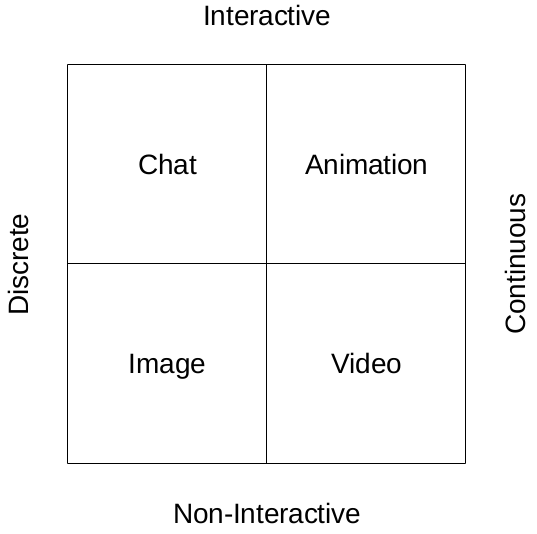
\includegraphics[width=0.45\textwidth]{figures/media_types.png}
	\caption{Media Types}
\end{figure}

	Media Types can be distinguished by two criteria, the first one describes a media as discrete or continuous, the second one describes it as interactive or non-interactive. A discrete media is characterized by its type not depending from time, as continuous media depending from it. Interactive media is characterized by its state being changed by external events such as user interactions.

	For example, an image is non-interactive and discrete, for instance, a video is continuous and non-interactive. A simple collaborative editor with just text is interactive and discrete. An animation that changes in function of user behavior is interactive and continuous.

	Streaming protocols like \ac {RTP} were designed for continuous and non-interactive media types, such as audio and video. Discrete and non-interactive media don't need to be streamed through \ac{RTP} because they don't change with. For example, if an image appears in a specific time interval, just the \ac{HTML} or \emph{JavaScript} that will reference the image must be streamed, the image itself is then transferred through \ac{HTTP}.

	In order to play any kind of stream, a player for interactive stream is needed for downloading an environment, decoding the \ac{RTP} payload to determine the state and display it to the user. Streaming interactive media like the combination of \ac{HTML}, \ac{CSS} and JavaScript require more than interpreting the code, a streamed user interface may contain an internal state that is not shown on code.

	Every time an event is processed on one of the endpoints, both sender and receivers state must stay synchronized, otherwise events may behave differently.

	To achieve synchronization of interactive data most packets have three types: \emph{State}, \emph{Delta-State} and \emph{Event}. State packet defines the environment complete state. Delta-State packets transports just the piece of state that changed. Event packets informs that an event occurred over the interactive media. 


	An \ac{RTP} recorder can have two operation modes, recording or playback. Traditional \ac{RTP} players can do random access, in contrast, interactive \ac{RTP} players must restore the environment and context at a given time. The environment is the initial state, so we can call it a non-interactive discrete media and handle it over \ac{HTTP}. After the receiver has received the environment, it should calculate the state at the given time. 

	If the \ac{RTP} recorder controls the correct data to send to the receivers, it cannot be a simple \ac{RTP} recorder as it must compute the state or delta-state to send. Therefore, if the receiver receives all recorded packets, it can calculate the current state from the previous complete state. Streaming too much complete states, results on more precise random accesses, but the trade-off is the higher bandwidth usage and used storage space on the recording server. On the other hand, if there are fewer complete states recorded followed by delta-states, the recorded stream will occupy less storage space, but random accesses will be less granular.

	It is possible to restore the media state even if messages are lost by recording and streaming the interactive media's complete state periodically.

	In order to synchronize an interactive application state amongst participants, the needed objects to synchronize must be serializable and sent to other participants.

  {\color{fade}[Model View Controller (Suited for interactive RTP)]}

	With such an interactive \ac{RTP} recorder it is then possible to record, play, fast forward, fast rewind, stop and jump to random positions.

  \cite{interactive_stream} proposed an \ac{RTP} profile for real-time transmission of interactive media. This new profile reuses much of video and audio profile implementation, integrating the interactive component.   \cite{interactive_record} explained how to record interactive video with this new profile.
	
	Multi-party video calls can be achieved on \ac{WebRTC} by streaming video from each participant to all the other participants. Although this works, the bigger a conference room is, the bigger is the bandwidth used to stream video to all participants within the conference room.

	\emph{Jitsi Video Bridge} \footnote{\url{http://jitsi.org/Projects/JitsiVideobridge}} receives one stream from every participant on a conference, either from a \emph{jitsi} client or a \ac{WebRTC} application, and redirects it to all the other conference participants, reducing the amount of data that each peer sends. Although all the participants need to download all the streams from \emph{Jitsi Video Bridge} server, typically download rates are much bigger than upload rates, making this solution more feasible.

	\emph{Jitsi Video Bridge} uses \ac{XMPP} as a signaling protocol and its \emph{colibri} extension \cite{xep0340} to reserve channels for video transmission. Although this choice for signaling protocol, \emph{Jitsi Video Bridge} also supports \ac{SIP}.

	\ac{OT} technology was originally developed for consistency maintenance and concurrency control over distributed objects, \ac{OT} algorithms are mainly used in collaborative applications such as distributed document edition.

	\emph{Google Wave} was a distributed collaboration platform based on \emph{Jupiter}\cite{jupiter} that adopted \ac{OT} techniques, other Google products such as Google Docs are using this type of technology. In 2010 Google stopped the development of Google Wave and released the main components as Open Source code to Apache, the project is currently known as \emph{Apache Wave} and the reference implementation is named as \emph{Wave in a Box}.

	\emph{ShareJS}\footnote{\url{http://sharejs.org/}} is an \ac{OT} \emph{JavaScript} library, developed by the ex \emph{Google Wave} engineer Joseph Gentle, for collaborative text and \ac{JSON} documents edition in real-time.

	\emph{TogetherJS}\footnote{\url{http://togetherjs.com/}} is a JavaScript library that uses \ac{WebRTC} for collaborative web applications. It uses \ac{JSON} messages for \ac{OT} concurrency control but it does not provide storage.

	\emph{Goodow}\footnote{\url{http://realtimeplayground.goodow.com/}} is a collaborative framework with its own server implementation, it supports four types of collaborative elements: String, Lists, Maps and Custom objects.
	


\section{Proposed Architecture}\label{arch} % English
  Taking into account the goals of this project and all the technology presented so far. Our proposal is the development of a web application that provides communication and collaboration in real-time.

The requirements for our web application are:

\begin{itemize}
 \item Enrich calls with any kink of multimedia in real-time.
 \item Ability perform tasks on real-time collaborative environment.
 \item Ability to record and playback interactive multimedia.
\end{itemize}

The infrastructure is composed by: Ice Server, Web Server, Stream Server, Signaling Server and Test Clients.

\begin{figure}[H]
	\centering
	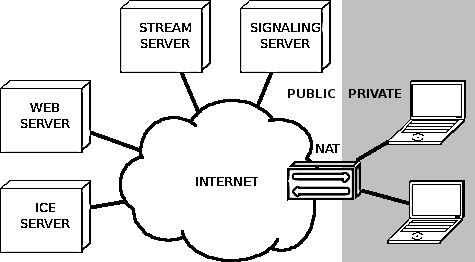
\includegraphics[width=0.55\textwidth]{figures/arch.png}
	\caption{System Architecture}
\end{figure}

Although the core infrastructure is important and crucial for the implementation of our web application, there is no preference for a specific software running on the web server. An important requirement for the Web Server is the WebSockets support, LAMP server was considered, although the chosen technology for web development is Play Framework with Java, which has a more evident separation between Model, View and Controller components.

For the signaling server there is also no preference between \ac{SIP} and \ac{XMPP}, as both support presence information feature. SigOFly could be adopted as well but using it would be irrelevant for the final result of this project. For sake of simplicity and easy deployment the chosen platform chosen is the Openfire \ac{XMPP} server.

The streaming server will be without any doubt \emph{Jitsi Videobridge} as \emph{Jitsi} team is working with \ac{WebRTC} and their code is open source.

The \ac{ICE} server is not required to be on our infrastructure as a public \ac{ICE} server could be used, if \ac{TURN} is used the network speed could drop due to resource share amongst other users. An \ac{ICE} server will be installed in order to prevent the influence of other users on our application.

On the client computers, both \emph{Mozilla Firefox} and \emph{Google Chrome} will be installed as web browsers. Libraries such as \emph{jQuery}, \emph{Bootstrap}, \emph{Strophe}, \emph{Modernizr} and \emph{TogetherJS} will be downloaded from the Web Server and executed on the client side.

\emph{Modernizr} and \emph{jQuery} will ensure that our application is compatible with the most popular web browsers.

\emph{Bootstrap} will be used to make user interface more appellative and responsive. With \emph{bootstrap} it's quite easy to develop applications that adapt to mobile devices with different screen sizes.

\emph{Strophe} library will be essential to communicate with \ac{XMPP} server and clients.

\emph{TogetherJS} will be used for the collaborative component of our web application, other libraries were considered but, as said before, \emph{TogetherJS} does not implement object storage making the object storage implementation free.

\section{Methodology}\label{meth} % Section



		%RP falta introdução à secção a explicar o que vai ser discutido aqui.
%RP texto que está nos 3 parágrafos seugintes ficava bem no planned schedule. Talvez esse fique melhor antes do evaluation methodology.
This section presents how we plan to implement and test our solution.

\subsection{Evaluation Methodology} % Section
	Our solution will be evaluated with several experiments, either qualitative and quantitative. 

Our web application will be tested with real users by asking them to perform some tasks, count the respective spent time and note their difficulties. After these tests, it will be suggested to users to fill out questionnaires. 

The results of user tests be used to improve the following prototype iterations, it is expected to notice both qualitative and quantitative improvements.

%RP elaborar o tipo de testes que vais fazer com os utilizadores: pedir para fazer tarefas e cronometrar o tempo que demoram. preencher questionários, decobrirem sozinhos como fazer algo, fazer após explicações, etc.

%RP detalhar os testes de desempenho de que falas.
 
The system in general will be validated with benchmarks that will focus on application delay when performing heavy tasks such as sharing a file and editing it in collaboration with other users. The amount of users will gradually increase in order to understand how much the performance degrades. 



	\subsection{Planned Schedule} % English
		\tikzset{every picture/.style={xscale=0.51,yscale=0.51,transform shape}}




\begin{ganttchart}[vgrid, hgrid]{1}{36}
\gantttitle{2015}{28}
\gantttitle{2016}{8} \\
\gantttitle{Jun}{4}
\gantttitle{Jul}{4}
\gantttitle{Aug}{4}
\gantttitle{Sep}{4}
\gantttitle{Oct}{4}
\gantttitle{Nov}{4}
\gantttitle{Dec}{4}
\gantttitle{Jan}{4}
\gantttitle{Feb}{4} \\
\gantttitlelist{1,...,36}{1}\\
%First Group
\ganttgroup{Thesis}{1}{32} \\
\ganttbar{Related work evaluation}{1}{28}\\
\ganttbar{Essay writing}{19}{32} \\
\ganttbar{Paper writing}{25}{32} \\
\ganttmilestone{Delivery}{35}{35} \\
%\ganttlink{elem0}{elem1}
%\ganttgroup{Resume}{1}{10} \\

%\ganttmilestone{Milestone 1}{11}
%Second Group
\ganttgroup{Implementation}{1}{1}\ganttgroup{}{4}{8}\ganttgroup{}{11}{26}\ganttgroup{}{29}{30} \\
\ganttbar{Basic configuration}{1}{1} \\
%\ganttlink{elem4}{elem5}
%\ganttmilestone{Milestone 1}{11}
%Third Group
\ganttbar{WebRTC basics}{4}{4} \\
\ganttbar{Video \& Audio Communication}{4}{5} \\
\ganttbar{Non-Interactive Record \& Playback}{6}{8} \\
\ganttbar{Interactive Record \& Playback}{11}{14}\\
\ganttmilestone{First Prototype}{18}\\
\ganttbar{Collaborative Environment}{15}{18}\\
\ganttmilestone{Second Prototype}{22} \\
\ganttbar{Interface Improvement I}{19}{22} \\
\ganttbar{Usability Tests I}{23}{23} \\
\ganttmilestone{Third Prototype}{25} \\
\ganttbar{Interface Improvement II}{24}{25} \\
\ganttbar{Usability Tests II}{26}{26} \\
\ganttbar{Performance Tests}{29}{30} \\
\ganttbar{Performance Improvements}{30}{30} \\
\ganttmilestone{Final Prototype}{30}

%\ganttlink{elem8}{elem9}


\ganttlink{elem9}{elem10}
\ganttlink[link type=F-S]{elem11}{elem12}
\ganttlink{elem12}{elem13}
\ganttlink[link type=F-S]{elem13}{elem15}
\ganttlink[link type=F-S]{elem15}{elem17}
\ganttlink[link type=F-S]{elem17}{elem18}
\ganttlink[link type=F-S]{elem18}{elem20}
\ganttlink[link type=F-S]{elem20}{elem21}
\end{ganttchart}


\section{Conclusions}\label{concl} % English


\subsection{Summary} % English
Neste secção deve-se fazer o resumo do trabalho efectuado, retomando a ideia, as contribuições definidas e a forma como estas se materializaram

\subsection{Conclusions} % English
Nesta secção devem ser retiradas conclusões do trabalho realizado, em face dos resultados obtidos \cite{exemplo}.


\bibliographystyle{splncs03}
\bibliography{references}

\end{document}
